\documentclass[tikz]{standalone}
\usetikzlibrary{calc,trees,positioning,arrows,chains,shapes.geometric,%
    decorations.pathreplacing,decorations.pathmorphing,shapes,%
    matrix,shapes.symbols,fit}

\pgfdeclarelayer{back}
\pgfsetlayers{back,main}


\makeatletter
\tikzset{
  fitting node/.style={
    inner sep=0pt,
    fill=none,
    draw=none,
    reset transform,
    fit={(\pgf@pathminx,\pgf@pathminy) (\pgf@pathmaxx,\pgf@pathmaxy)}
  },
  reset transform/.code={\pgftransformreset}
}
\makeatother


\begin{document}
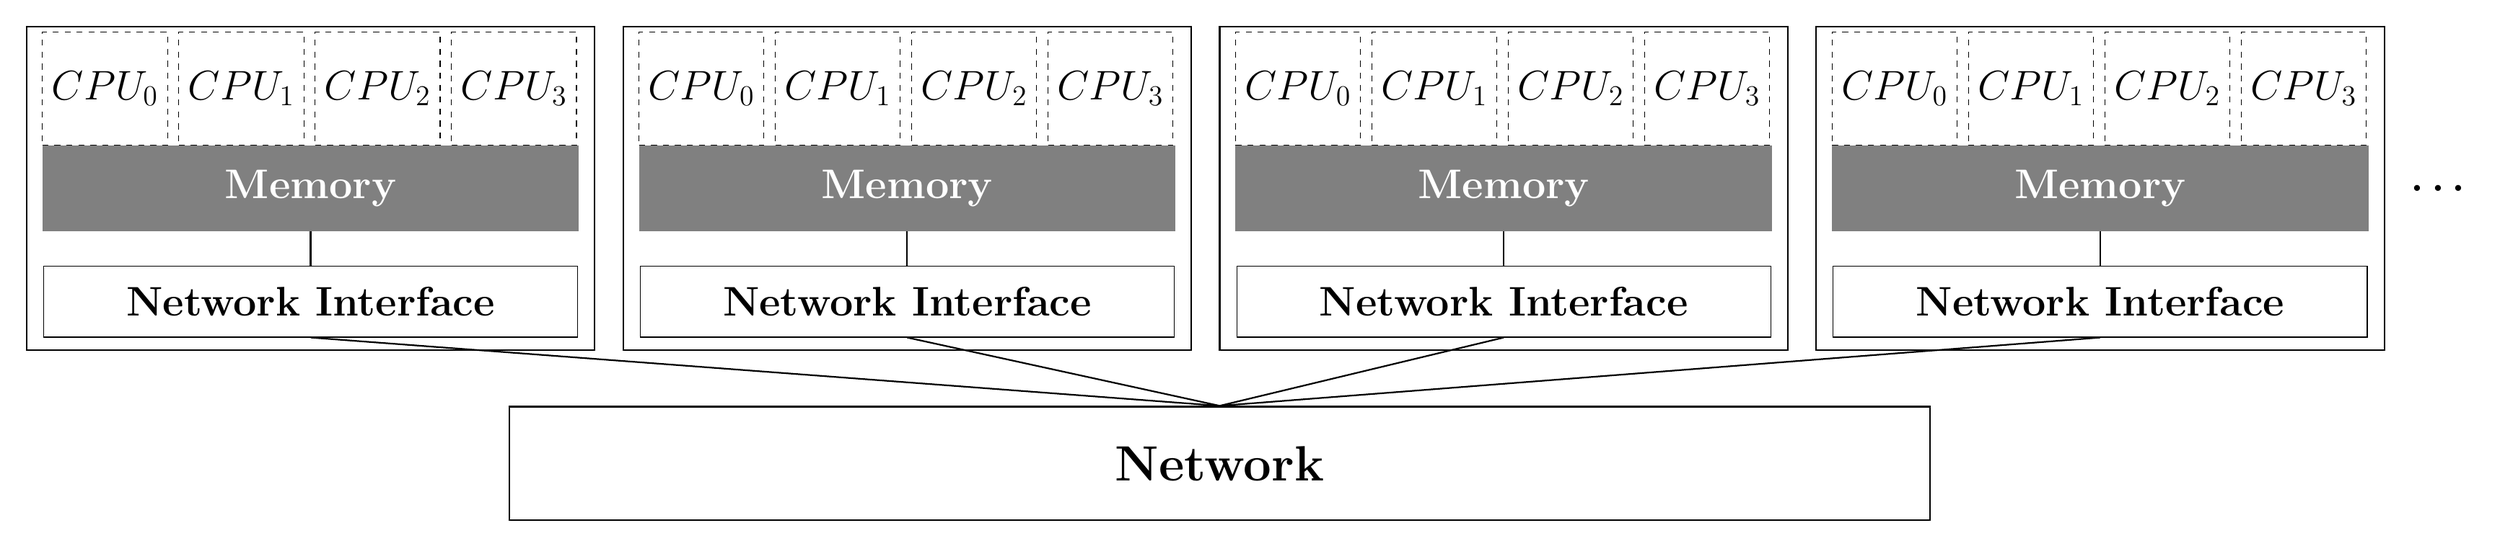
\begin{tikzpicture}

  \node [draw,thick,rectangle, minimum width=25cm, minimum height=2.cm,font=\Huge] at(21,-2) (switch) {\bfseries{}Network};

  \foreach \n in {0,...,3}
  {

    \node at($(0,0)+(10.5*\n,0)$) (cpu_anchor_sw) {}; 
    \node at($(cpu_anchor_sw)+(10,5.7)$) (cpu_anchor_ne) {}; 

    \draw[thick] ($(cpu_anchor_sw)$) rectangle ($(cpu_anchor_ne)$) node[fitting node] (cpu_envelope_\n) {};
    
    \draw[-,fill=gray,draw=gray] ($(cpu_envelope_\n.west)+(.3,-.75)$) rectangle ($(cpu_envelope_\n.east)+(-.3,.75)$) node[fitting node] (meminterface) {};
    \node (meminterface_label) [text=white,font=\huge] at(meminterface) {\bfseries{}Memory};

    \node [draw,rectangle, minimum width=9.4cm, minimum height=1.25cm,font=\huge] at($(meminterface)+(0,-2)$) (nic) {\bfseries{}Network Interface};

    \draw[thick] ($(nic.north)$) -- ($(meminterface.south)$) {};
    \node (cpu_anchor) at($(meminterface.north west)+(1.1,1)$) {};  

    \foreach \c in {0,...,3}
    {
      \node [draw,dashed,rectangle, minimum width=2.2cm, minimum height=2cm,font=\huge] at($(cpu_anchor)+(2.4*\c,0)$) {$CPU_\c$};
    }

    \draw[thick] ($(nic.south)$) -- ($(switch.north)$)  {};
  }

  \node [font=\huge] at($(cpu_envelope_3.east)+(1,0)$) (cpu_anchor_sw) {\bfseries{}\dots}; 
\end{tikzpicture}
\end{document}
